%----------------------------------------------------------------------------------------
%	PACKAGES & THEMES
%----------------------------------------------------------------------------------------

\documentclass[8pt]{beamer}

\usepackage{etex}
\mode<presentation> {
\usetheme{Vilanova}
}

\usepackage[english]{babel}
\usepackage[utf8]{inputenc}
\usepackage{array}
\usepackage{graphicx}
\usepackage{booktabs}
\usepackage{amsmath,amssymb,amsthm}
\usepackage{xcolor}
\usepackage{tikz}
\usetikzlibrary{arrows}
\usepackage{pifont}
\usepackage{listings,color}
\usepackage{import}

\definecolor{listcomment}{rgb}{0.0,0.5,0.0}
\definecolor{listkeyword}{rgb}{0.0,0.0,0.5}
\definecolor{listnumbers}{gray}{0.65}
\definecolor{listlightgray}{gray}{0.955}
\definecolor{listwhite}{gray}{1.0}

\AtBeginSection[]
{
\addtocounter{framenumber}{-1}
\begin{frame}
\frametitle{Outline}
\tableofcontents[currentsection]
\end{frame}}

%----------------------------------------------------------------------------------------
%	TITLE PAGE
%----------------------------------------------------------------------------------------
\title{Remote Sensing Image Processing}
\subtitle{What's new in Orfeo ToolBox?}
\author{Julien Michel (CNES)}
\date{Foss4g Europe 2018, July 16th-21th 2018, Guimarães}

\pgfdeclareimage[height=96mm,width=128mm]{background}{../OTB-General/images/fondsClairSansLogo}
\pgfdeclareimage[height=0.2cm]{cc}{../OTB-General/images/CC-licence.png}
\setbeamertemplate{background}{\pgfuseimage{background}}
\pgfdeclareimage[height=0.6cm]{logoIncrust}{../OTB-General/images/logoIncrust}
\pgfdeclareimage[height=0.6cm]{OSGeo_logo}{../OTB-General/images/OSGeo_logo}
\logo{
\begin{tabular}{p{0.22\textwidth}p{0.58\textwidth}p{0.1\textwidth}p{0.1\textwidth}}
\href{http://www.osgeo.org}{\pgfuseimage{OSGeo_logo}}
& \vspace{-0.03\textwidth} \scriptsize{} % date and event here
& \href{http://creativecommons.org/licenses/by-sa/3.0/}{\pgfuseimage{cc}} & \href{http://www.orfeo-toolbox.org}{\pgfuseimage{logoIncrust}}\\
\end{tabular}
}

\begin{document}
\begin{frame}
\titlepage
\end{frame}

\mode<all>
\subimport{../OTB-General/}{introduction-en.tex}

\mode<all>
\subimport{../OTB-General/}{images.tex}

%% \mode<all>
%% \subimport{../OTB-General/}{key-characteristics-en.tex}

\mode<all>
\subimport{../OTB-General/}{howto_use-en.tex}

\mode<all>
\subimport{../OTB-General/}{releases/otb-qgis-en.tex}

\mode<all>
\subimport{../OTB-General/}{remote-modules-en.tex}

\section*{Conclusion}

\begin{frame}{Conclusion}

  \begin{block}{What you learned}
    \begin{itemize}
      \item What OTB can do for you (incomplete)
      \item How to use OTB
    \end{itemize}
  \end{block}
  
  \begin{block}{Take home message}
    \begin{itemize}
    \item We are comitted to make OTB in QGis better
    \item Remote modules are a standard way to package and share OTB code
    \item Interesting new features (even full processing chains) as remote modules
    \end{itemize}
  \end{block}

  \begin{block}{Future}
    \begin{itemize}
      \item Big changes for OTB 7.0
      \item Enhance further python API
      \item More amazing remote modules
      \item \url{gitlab.orfeo-toolbox.org/orfeotoolbox/otb/issues}
    \end{itemize}
  \end{block}
\end{frame}

\begin{frame}
  \frametitle{OTB Users Day 2018 - Montpellier - 19/10/2018}
  \begin{description}
  \item[Where?] \href{http://www.agropolis.fr/pratique/locaux.php}{Agropolis International}
  \item[When?] 19 Octobre 2018 - Following Theia Symposium \href{http://theia2018.sciencesconf.org}{THEIA}
  \item[What?] Talks, feedback, training, brainstorming ...
  \item[How?] Free, open to everyone!
  \item[Register!] \url{https://tinyurl.com/y7yzjvad}
  \end{description}
  \begin{center}
    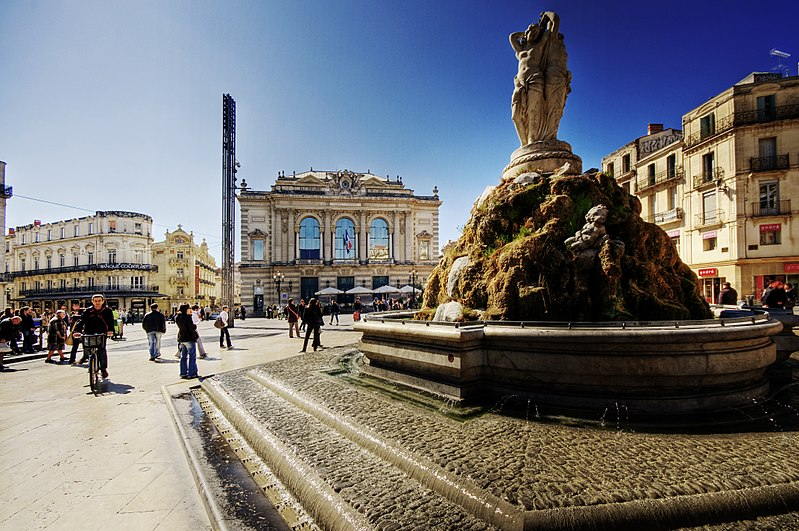
\includegraphics[width=0.45\textwidth]{../foss4gfr-2018/images/montpellier.jpg}
  \end{center}  
\end{frame}


\end{document}
